\section{Methodology}
  \textbf{Problem Formulation}\\
  Given a car in a 2D map with predetermined start point and end point and circular obstacles that have randomly generated radius. The goal of the project is to introduce a collision-free Path Planning Algorithm and a Trajectory Tracking method to guide the car along the path.
  The factor that we are trying to minimize is the danger of the Bezier path. The closer the path is relative to the obstacles, the more danger the path yields.

  \subsection{Path Planning Algorithm}
  The Path Planning Algorithm involves the presence of Artificial Potential Field, Bezier Curve and most importantly, Genetic Algorithm. The general training procedure of our model can be described as follows:
  \begin{enumerate}
    \item \textbf{Introduce a Bezier to Chromosome encoding strategy:} The encoding scheme is a universal definition of the chromosome and any latter functionality, model training procedure will have to surround this definition.
    \item \textbf{Determine a general definition of path's danger:} Artificial Potential Field will present in this part, help generating tools needed to evaluate the chromosomes latter on.
    \item \textbf{Initialize the first population}: Create random initial chromosomes.
    \item \textbf{Artificial selection}: Artificial Fitness Function is defined and will be complimented with APF to evaluate the population.
    \item \textbf{Artificial evolution}: The population will undergo the crossover and mutation, mimicking the natural evolution of animals and organisms.
    \item \textbf{Loop}: Return to step 4 until the number ofatraining epoch runs out.
  \end{enumerate}

  \subsubsection{Bezier to Chromosome Encoding Strategy}
  The chromosomes of the Genetic model is defined as a sequence of control points of the Bezier Curve which will act as genes.
  For instance, a curve that has $P_0$, $P_1$, $P_2$ and $P_3$ as control points will be encoded into $\mathbf{P}=\{P_0, P_1, P_2, P_3\}$ as chromosome.
  Since the start and end positions of the car on the 2D map are known, we will assign the first and last control points in the sequence corespond with them, which means the sequence $\{P_0, P_1, P_2, P_3\}$ will become $\{P_S, P_1, P_2, P_E\}$.
  \begin{figure}[H]
    \centering
    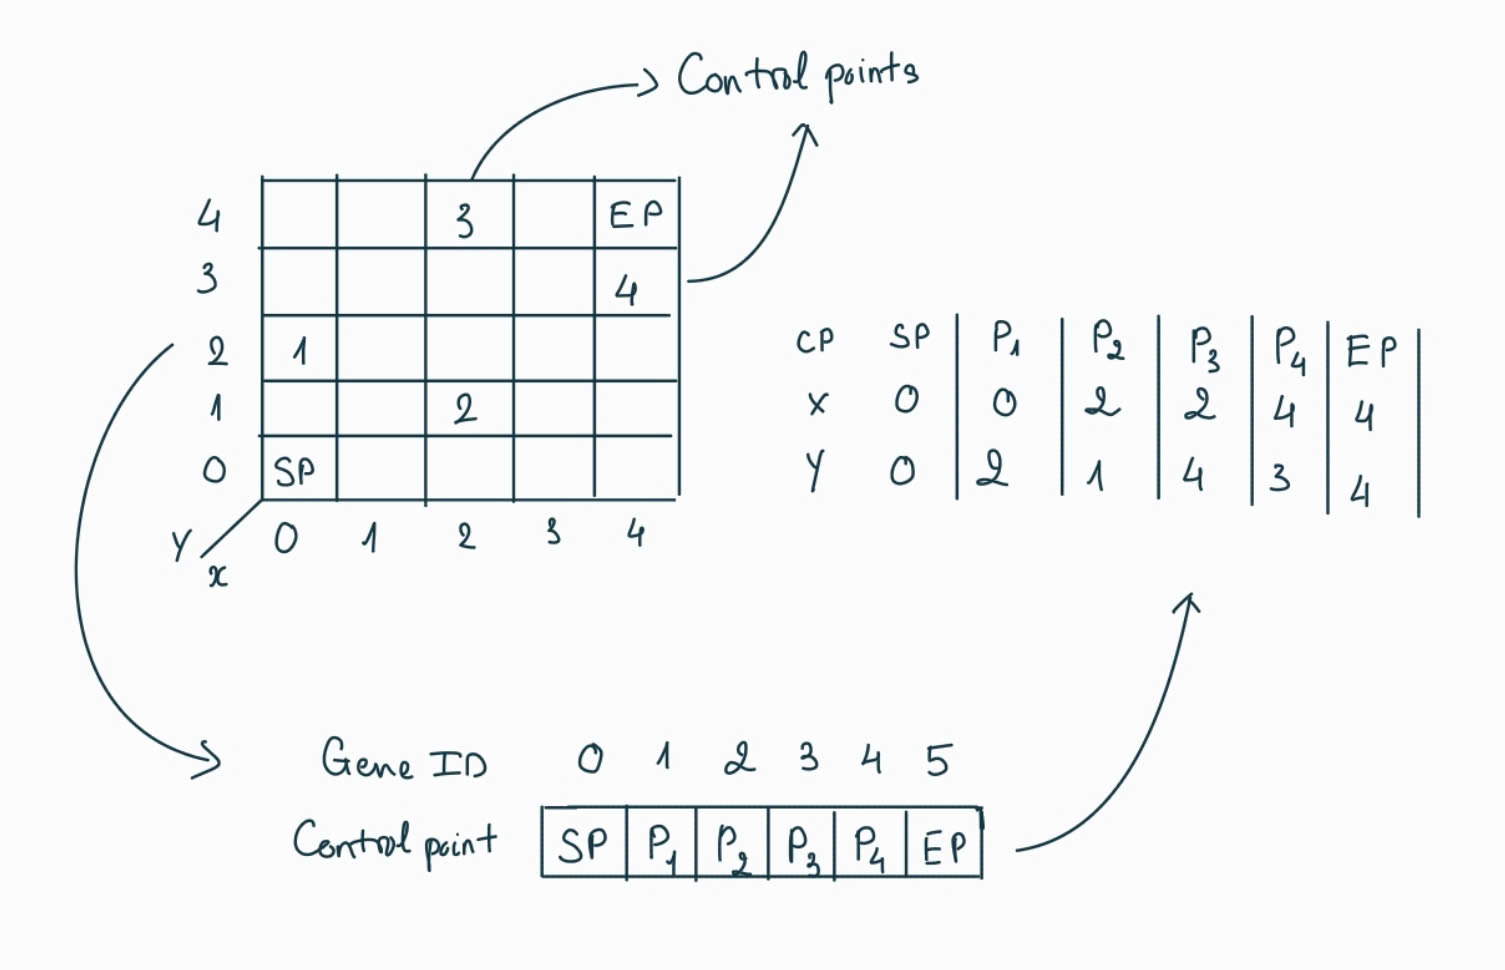
\includegraphics[width=0.8\textwidth]{chromosome_encoding.jpg}
    \caption{Chromosome Encoding Strategy}
  \end{figure}

  \subsubsection{Danger Map Generation}
  For the static 2D map with size $H\times W$, with $H$ and $W$ are the height and width (in pixels) of the map respectively, we will compute the level of danger of each pixel on the map based on its distance from all surrounding obstacles
  \begin{itemize}
    \item $ (x, y) $: Coordinates of a pixel.
    \item $ (O_{x,i}, O_{y,i}) $: Coordinates of the $ i $-th obstacle's center.
    \item $ r_i $: Radius of the $ i $-th obstacle (fully dangerous region).
    \item $ S $: Vehicle size.
    \item $ R_i = r_i + S $: Outer limit radius for the $ i $-th obstacle.
    \item $ d_i(x, y) = \sqrt{(x - O_{x,i})^2 + (y - O_{y,i})^2} $: Distance between the pixel $(x, y)$ and the $ i $-th obstacle.
    \item $ D_i(x, y) $: Danger level contribution from the $ i $-th obstacle.
  \end{itemize}
  The contribution of each obstacle to the danger level is calculated as follows:
  $$
    D_i(x, y) =
    \begin{cases} 
      1, & \text{if } d_i(x, y) \leq r_i, \\
      1 - \frac{\log_{10}(d_i(x, y) - r_i)}{\log_{10}(R_i - r_i)}, & \text{if } r_i < d_i(x, y) \leq R_i, \\
      0, & \text{if } d_i(x, y) > R_i.
    \end{cases}
  $$
    
    \subsubsection*{Cumulative Danger Level}
    
    The total danger level at a pixel $(x, y)$ is the sum of danger level from all obstacles:
    $$D(x, y) = \min\left(\sum_{i=1}^{N_{obs}} D_i(x, y), 1\right)$$
    where $N_{obs}$ is the total number of obstacles.


  \subsubsection{Initialize Population}
  At the start of the training procedure, an initial population needs to be generated.
  The number of individuals or population size $C$ will be fixed throughout the training procedure.
Each chromosome contains some initial amount of random genes.

  \subsubsection{Fitness Function}
  We defined the fitness values of the each chromosomes be the average danger level over the associated Bezier Curve by taking the line integral and then divided by the curve's length.
  $$\mathbf{P}\Rightarrow B(t)$$
  $$f_{fit}(B(t))=\frac{\oint_LD(B(t))dl}{L}=\frac{\int_0^1D(B(t))dt}{L}$$
  where
  \begin{itemize}
    \item $B(t)$ is the Bezier curve parametric equation with respect to $t$ converted from $\mathbf{P}$ which yields the coordinate of the local point with specific value of $t$
    \item $L$ is the length of the Bezier curve
  \end{itemize}
  In computer programming, the finess values can be calculated by replacing the line integral with the sum of danger values of each discrete local point on the Bezier Curve divided by the number of points that we are calculating with.
  First, we create $N_{bres}$ number of evenly spaced t values from ranging from 0 to 1. It is called "Bezier Resolution".
  $$\mathbf{t}=\{0, 1\times\frac{1}{N_{bres}}, 2\times\frac{1}{N_{bres}}, 3\times\frac{1}{N_{bres}},..., (N_{bres}-1)\times\frac{1}{N_{bres}},1\}$$
  After that, the average danger level of each chromosomes can be calculated as follows:
  $$
  f_{fit}=
  \begin{cases} 
    1,  \text{if } \exists O_i \text{ that } \left\lVert P_B(O_i) - O_i \right\rVert \leq r_i \\
    \frac{1}{N_{bres}}\sum_{i=0}^{N_{bres}}D(\lfloor B(t_i) \rfloor)
  \end{cases}
  $$
  The highest possible fitness value (most inefficient chromosome) returned is 1 when the chromosome crosses an obstacle.
  The $\lfloor B(t_i) \rfloor$ operation is used to round down the point's position, calculate the nearest pixel with integer value since the parametric equation yields floating point values.
  The function $P_B()$ is used to find the current point's projection on the Bezier Curve, which we will define later in the Trajectory Tracking section.\\
  After running through the finess function, the chromosomes will be separated into 2 groups: elites (fitness values $< T_S$) and non-elites (the rest) with $T_S$ is the Separation Threshold.
  
  \subsubsection{Crossover and Mutation}
  \subsubsection*{Crossover}
  The crossover process will then be performed separately on 2 groups: elites and non-elites.
  In each group, we will select a proportion $R_C$ (crossover ratio) of chromosomes to perform crossover. The process is defined as randomizing a crossover position on the interval $\left[0; min(L_{\mathbf{P_A}}, L_{\mathbf{P_B}})\right]$ with $L_\mathbf{P_A}$ and $L_\mathbf{P_B}$ are the lengths of 2 parent chromosomes respectively since the length of chromosomes throughout the training procedure may vary.\\
After that, the genes behind the crossover position of the 2 parental chromosomes will be exchanged.
  \begin{figure}[H]
    \centering
    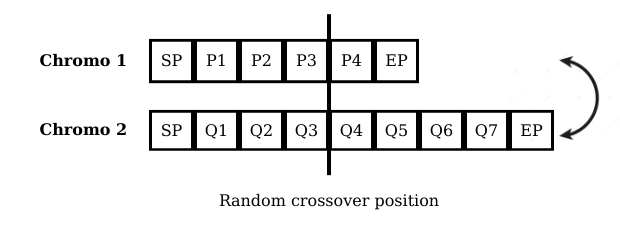
\includegraphics[width=0.8\textwidth]{crossover.png}
    \caption{Crossover mechanism}
  \end{figure}

  \subsubsection*{Mutation}
  There are three types of mutation going to be used: add gene, remove gene and edit gene. The mutation process will be conducted only on a small proportion named Mutation Ratio $R_M$ of the non-elite chromosomes. The mutation position will also be randomized.
  \begin{figure}[H]
    \centering
    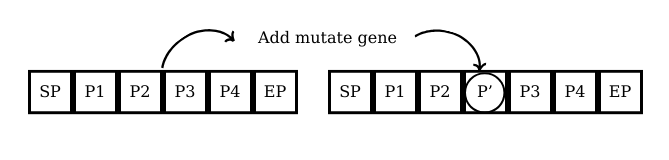
\includegraphics[width=0.7\textwidth]{add_gene.png}
    \caption{Add gene}
  \end{figure}
  The additional gene will be randomized in the scope of the map size
  \begin{figure}[H]
    \centering
    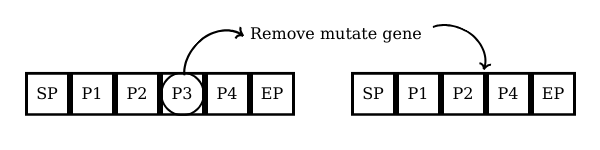
\includegraphics[width=0.7\textwidth]{remove_gene.png}
    \caption{Remove gene}
  \end{figure}
  Randomly select a gene to be removed from the chromosome
  \begin{figure}[H]
    \centering
    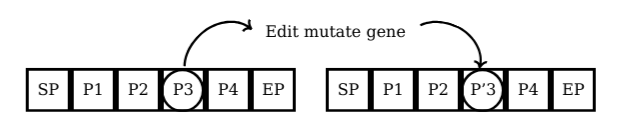
\includegraphics[width=0.7\textwidth]{edit_gene.png}
    \caption{Edit gene}
  \end{figure}
  The chosen gene will be re-randomized in the scope of the map size.

  \subsubsection{Overal Algorithm Workflow}
  \begin{figure}[H]
    \centering
    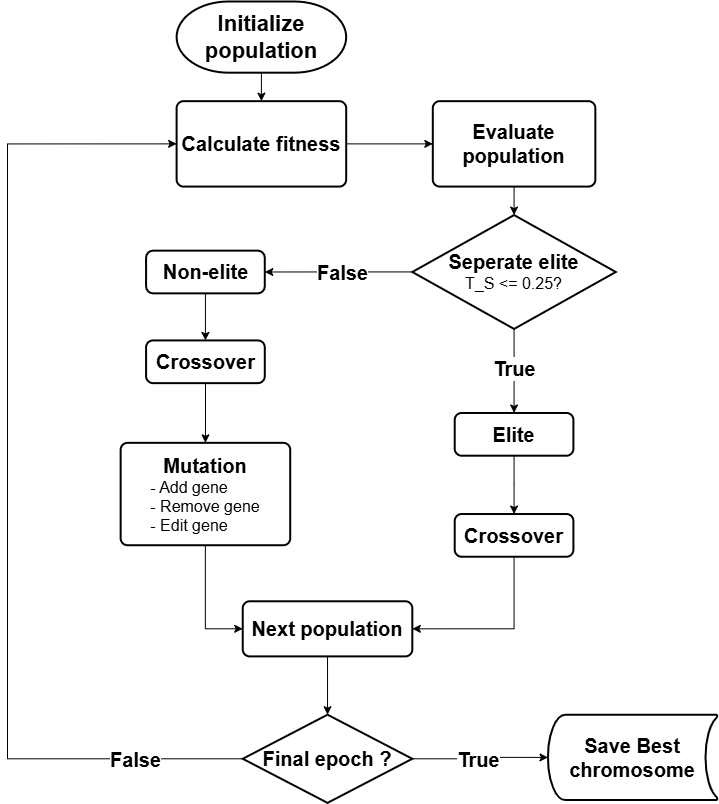
\includegraphics[width=0.55\textwidth]{genetic_model.png}
    \caption{Algorithm Workflow}
  \end{figure}

  \subsection{Trajectory Tracking Algorithm}
  The algorihm we introduce uses PID Controller with and the supporting Binary Search Algorithm to hhelp the car stays on track throughout the collison-free motion.
  There are several aspects need to be handle in order:
  \begin{enumerate}
    \item \textbf{Introduce the vehicle's model:} Propose the 2D motion of the car mathematically.
    \item \textbf{Load the path}: The procedure starts by loading the best chromosome saved in the local memory that has been trained from the Genetic Model earlier.
      Then the chromosome will need to be converted into the Bezier Curve
    \item \textbf{Control loop:}
      \begin{itemize}
        \item Find the car's projection on the Bezier Curve
        \item Calculate error
        \item Calculate PID
        \item Update vehicle's state
      \end{itemize}
  \end{enumerate}
    % \item \textbf{Considering noise in the simulation:} Since the vehicle's motion in simulation environment is described mathematically with equations so the car's behavior is completely perfect.
      % However, in the real-life scenarios, physical vibrations and errors are inevitable.
      % These factors, therefore, need to be considered in the vehicle's mathematical model to prove that our approach is effective.

    \subsubsection{Vehicle model}
    The general motion equation of the car can be expressed with a set of equations:
    $$X(t)=\int_0^tV_{car}\cdot\vec{u}(t)dt$$
    $$\vec{u}(t):=R(\omega(t)dt)\cdot\vec{u}(t)$$
    where:
    \begin{itemize}
      \item $\vec{u}(t)$ is a unit vector, representing the direction that the car is currently heading.
      \item $
        R(\alpha)= \begin{bmatrix}
          cos(\alpha) & -sin(\alpha) \\
          sin(\alpha) & cos(\alpha)
        \end{bmatrix}
      $ is the rotation matrix.

    \end{itemize}
    The position of the car with respect to time $X(t)$ is obtained by continously integrating velvelocity $V_{car}\cdot\vec{u}(t)$ with respect to time.
    To further simplify the problem, we define the speed of the car to be constant, hence the equation becomes:
    $$X(t)=X_0+V_{car}\cdot\vec{u}(t)dt$$
    The heading vector $\vec{u}(t)$ at any time $t$ is determined by continuously rotating the vector itself from the beginning of the simulation. The $:=$ operation means assigning the value back to the variable.
    In order to control the car, helping the vehicle follow the generated path, the introduced PID algorithm is utilized to calculate the angular velocity $\omega_{pid}$ each control loop.
    \\
    However, in the simulated environment, all movements are represented through mathematical equations so the car would perform perfectly.
  In real-world scenarios, physical vibrations and inherent errors are inevitable.
  Therefore, incorporating these factors into the model is essential to validate the system's effectiveness.
  $$\omega(t)=\omega_{pid}+\omega_{\Omega}$$
  where $\omega_{\Omega}$ is the system noise produced that we formulate as a representation of real world vibrations and errors that obeys the Gaussian Distribution.
  $$\omega_{\Omega}=\eta\cdot x$$
  with
  $$\mathcal{N}(x|\mu,\sigma^2) = \frac{1}{\sigma\sqrt{2\pi}}e^{-\frac{1}{2}(\frac{x-\mu}{\sigma}})^2 $$
  where $\eta$ is the maximum value of the the angular velocity noise can ever be achieved. 
    
    \subsubsection{Initialization}
    \begin{itemize}
      \item \textbf{Initial population:} Generating $C$ chromosomes 
      \item \textbf{Car position:} Coinciding the starting position.
      \item \textbf{Car heading:} Facing toward the ending position.
      \item \textbf{Load terrain:} Loading map with obstacles have been pre-created earlier.
      \item \textbf{Load best chromosome:} Executing the control points position of the chromosomes with the lowest fitness score throughout the epoches.
      \item \textbf{Convert chromosome to Bézier path:} Convert the saved chromosome into Bezier Path.
    \end{itemize}
    \subsubsection{Control loop}
    \subsubsection*{Find projection}
    Determining the projection of a point on the Bezier Curve is the back bone principle of our PID control flow.
    Firstly, to minimize the computing time, we need to find a good starting point $B_{t_{mid}}$ on the curve before performing the Binary Search Algorithm by iterating over $N_{bres}$ $t$ values in $\mathbf{t}$.
    $$t_{mid} = \underset{t\in\mathbf{t}}{\arg\min}\(\left\lVert B(t) - K \right\rVert\)$$
    where $K$ is the point that we are trying to find projection of.
    \\
    Then we know for the fact that $B(t_{mid})$ is the closest point from K along the points in the Bezer resolution, the more optimal $t$ value that yields a more optimal solution must lies on the interval $\left[t_{mid}-\frac{1}{N_{bres}}; t_{mid}+\frac{1}{N_{bres}}\right]$.
    \\
    Let us define $t_{left} = t_{mid} - \frac{1}{N_{bres}}$ and $t_{right}=t_{mid}+\frac{1}{N_{bres}}$
    The algorithm works by repeatedly do the following operations in order:
    \begin{enumerate}
      \item Calculating the distance between K and the two middle points of the intervals $[t_{left};t_{mid}]$ and $[t_{mid};t_{right}]$
        \begin{center}
          $d_1 = \left\lVert B\left(\frac{t_{left}+t_{mid}}{2}\rigth)-K \right\rVert$ and 
          $d_2 = \left\lVert B\left(\frac{t_{mid}+t_{right}}{2}\rigth)-K \right\rVert$ 
        \end{center}
      \item Compare $d_1$ and $d_2$ to detemine which interval does the answer lies in
      \item Ignore the interval that doesn't have the answer then update the left and right boundaries by assigning new values to $t_{left}$ and $t_{right}$
        \begin{itemize}
          \item $t_{right} = t_{mid}$ and keep $t_{left}$ the same if $d_1<d_2$
          \item $t_{left} = t_{mid}$ and keep $t_{right}$ the same if $d_1\neq d_2$
        \end{center}
      \item Update $t_{mid} = \frac{t_{left} + t_{right}}{2}$
      \item Check termination condition and repeat step 1 if not satisfied.\\
        The we define a Termination Threshold $T_{BS}$ if $t_{right}-t_{left} \leq T_{BS}$ then the algorithm will yield the result $B(t_{mid})$
    \end{enumerate}
    

    \subsubsection*{Calculate error}

    \subsubsection*{Calculate PID}
    \begin{itemize}
      \item \textbf{Propotional(P):} Adjusting the control output in proportion to the error magnitude.The larger the error, the stronger the corrective action.\\
        $$P_{term}=P_I \cdot Y_{err}$$\\
      \item \textbf{Integral (I):} Addressing the accumulation of past errors. It is designed to eliminate steady-state errors that cannot be corrected by the proportional term alone.\\
        $$I_{term} = K_I \cdot \int_{0}^{t} Y_{err} \, dt$$
      \item \textbf{Derivative(D):} Predicting the future behavior of the error by considering its rate of change. This term helps to dampen oscillations and improve stability.\\
        $$D_{term} = K_D\cdot\frac{d Y_{err}}{dt}$$   
    \item \textbf{Control Variable $\omega_{\text{pid}}$}: Minimizing deviations from a desired target or setpoint.
        $$\omega_{\text{pid}} = K_P \cdot Y_{\text{err}} + K_I \cdot \int_{0}^{t} Y_{\text{err}} \, dt + K_D \cdot \frac{dY_{\text{err}}}{dt}$$
    \end{itemize}
    \subsubsection*{Update vehicle}
    \begin{itemize}
	    \item \textbf{Heading:} The heading vector, representing the vehicle's orientation, is rotated by an angle of ω plus a noise term to account for uncertainties or disturbances.\\
        $$\begin{bmatrix}
	        cos(\omega + \omega{\Omega}dt) & -sin(\omega + \omega{\Omega}dt) \\
    	    sin(\omega + \omega{\Omega}dt) & cos(\omega + \omega{\Omega}dt)
        \end{bmatrix}
        \cdot \vec{u}(t)$$\\
	    \item \textbf{Noise:} Introducing random disturbances into the vehicle's steering control by generating noise based on a normal distribution. This noise simulates the real-world unpredictability of vehicle dynamics and environmental effects.\\
		    $$\omega_{\Omega}=\eta\cdot x$$
	    \item \textbf{Position:} The vehicle's position is incremented in the direction of the updated heading vector, scaled by the vehicle's velocity and normalized by the frame rate. This step ensures the vehicle's movement is consistent with its velocity and the simulation's time resolution.\\
		    $$X(t)=X_0+V_{car}\cdot\vec{u}(t)dt$$
	    \item \textbf{Normalized heading:} After the heading is updated, it is normalized to maintain a consistent magnitude. This normalization ensures numerical stability and avoids issues caused by cumulative floating-point errors during repeated updates.\\
		    $$\dfrac{\vec{u}(t)}{\left\lVert \vec{u}(t)\right\rVert}$$
    \end{itemize}

